% !TeX spellcheck = da_DK
\section{Systembeskrivelse} 
Dette afsnit indeholder en beskrivelse af det system, der skal kunne anvendes af apopleksipatienter som et selvstændigt træningsapparat i rehabiliteringen af balanceproblemer. Systembeskrivelsen indeholder målgruppen for designet, samt hvilket formål og anvendelse det har. Ud fra disse faktorer er systemet blevet designet og illustreret i et blokdiagram. 

\subsection{Systemets bruger}
Systemet udvikles til apopleksipatienter med balanceproblemer mhp. selvtræning af balance i rehabiliteringsfasen, der bliver omtalt som fase 3 og 4 i afsnit \ref{Faser} på side \pageref{Faser}. Jævnfør afsnit \ref{Indledning} på side \pageref{Indledning} ses det, at majoriteten af apopleksipatienter er over 65 år, og systemet skal derfor være let anvendeligt. Systemets design skal altså være enkelt, så der ikke skabes forvirring blandt brugerne ift. systemets funktioner. Fagkyndigt personale, såsom fysioterapeuter og læger, skal kunne instruere patienten i brugen af systemet samt følge med i udviklingen, som patienten gennemgår. Det skal derfor være muligt for det fagkyndige personale at anvende systemet og aflæse data herfra. 
%Dette gøres ved at have et analogt og digitalt output, hvor den digitale del henvender sig til det fagkyndige personale i form af grafer, mens den analoge del henvender sig til apopleksipatienterne. \fxnote{Erikas kommentar: relevans ift. analogt og digitalt output? Tekniske detaljer! Er det vigtigt, at det er et analog output eller at det output indeholder specifik information?}   

\subsection{Systemets formål og anvendelse}
Systemets input er patienternes kropshældning, dvs. hvor meget vedkommende svajer i det frontale plan, i anatomisk position og under udførelse af en bestemt øvelse kaldet Sharpened Rombergs Test (SRT). Systemet skal kunne konvertere informationerne vedrørende patienternes kropshældning til visuel og somatosensorisk feedback samt et digitalt output i form af grafer. Den visuelle og somatosensorisk feedback har til formål at gøre apopleksipatienter opmærksomme på, hvornår de har bevæget sig over den normale grænse for krops svaj. Således kan systemet registrere, hvis patienten er i risiko for at falde. Inden et fald sker, udsendes et feedback signal, så patienterne har mulighed for at rette sig op. Selve systemet skal anvendes til selvtræning i hjemmet. Det skal derfor være et brugervenligt system, dvs. systemet skal kunne påsættes uden problemer og fungere uden, at patienten skal navigere rundt i forskellige funktioner for at påbegynde feedbacken. Systemet skal fungere som en hjælp for patienten, da vedkommende bliver bevidst omkring sin balance. Herved kan apopleksipatienten være mere selvstændig i rehabiliteringsprocessen.

Systemet designes til selvtræning af statisk balance. Patienterne kan anvende systemet ved to sværhedsgrader ift. kropsposition: normal kropsstilling (anatomisk udgangsposition) og øvelsen SRT. Apopleksipatienternes balance udfordres i højere grad af SRT end ved normal kropsstilling, eftersom kropsvægten fordeles anderledes ved denne øvelse ift. den normale kropsstilling omtalt i afsnit \ref{BalanceAfsnit} på side \pageref{BalanceAfsnit}. SRT udføres i stående udgangsposition med fødderne på en tegnet linje, så den ene fods tæer er mod den anden fods hæl. Derudover holdes armene tæt ind til kroppen og over kors. \cite{Huo1999}.\\ %Denne position er valgt for at udfordre patientens balance ved at fordele kropsvægten anderledes ift. den normale kropsstilling omtalt i afsnit \ref{BalanceAfsnit} på side \pageref{BalanceAfsnit}. % Patienten påsætter selv systemet øverst på sternum og udfører herefter en kort prøvetest for at kende til de givne feedback parametre.Under prøvetesten svajer patienten langsomt fra side til side. 
%Det er på baggrund af afsnit \ref{MekBioFeed} på side \pageref{MekBioFeed} valgt at hældningen på patienten skal opfanges vha. et accelerometer, der er placeret øverst på sternum. 
Det er på baggrund af afsnit \ref{MekBioFeed} på side \pageref{MekBioFeed} valgt, at systemet skal placeres øverst på sternum for at få bedst mulige målinger ift. patienternes kropshældning. Systemet skal give visuel og somatosensorisk feedback i form af en vibrator samt fem dioder bestående af en grøn, to gule og to røde. Som nævnt i afsnit \ref{BalanceAfsnit} på side \pageref{BalanceAfsnit} er grænsen for, hvornår et fald forekommer ift. hældningsgrad individuel. I praksis bør systemet dermed tilpasses til den enkelte patient på baggrund af testøvelser ift. balancen. Hældningsgraderne vil i dette projekt blive valgt på baggrund af raske forsøgspersoner, da det vurderes udfra problemanalysen afsnit \ref{BalanceAfsnit} side \pageref{BalanceAfsnit}, at apopleksipatienter har flere sygdomsrelaterede faktorer, der kan påvirke deres hældningsgrad. Hvis patienten hælder i intervallet $8^{\circ}$-$13^{\circ}$ til højre, indikeres dette af den gule diode på højresiden af den grønne diode. Derudover aktiveres en mild vibration, når den gule diode lyser. Hvis patienten hælder $13^{\circ}$ eller derover, lyser den røde diode til højre for den gule diode og styrken af vibrationen forøges. Det samme gør sig gældende for hældning mod venstre. Med denne metode indikeres både, hvilken retning patienten svajer samt graden heraf. Ved benyttelse af to feedback former er der større mulighed for, at patienten kan opfange signalerne. Hvis patientens visuelle sans er begrænset kan systemet stadig benyttes grundet den somatosensorisk feedback. \\ 
Efter en test af systemet udføres selve træningsøvelsen, hvor den valgte udgangspositionen ift. sværhedsgrad indtages på linjen. For at øge sværhedsgraden yderligere kan den visuelle sans udelukkes. Patienten skal under øvelsen forsøge at holde balancen så længe som muligt uden at bevæge sig ud i risikozonerne. Hvis patienten kommer ud i risikozonerne, vil dette blive markeret ved lys i dioderne samt vibration. Træningsøvelsen kan gentages efter behov. Ved at tage flere målinger igennem rehabiliteringsforløbet vil det forventes, at der sker en fremgang ift. tiden, hvori balancen kan opretholdes uden at patienten bevæger sig ud i risikozonerne. 

\subsection{Accelerometer}
Der er valgt et accelerometer til måling af det biologiske signal, som der skal gives feedback på. Accelerometeret ADXL335, som ses på \figref{ADXL335} er en treakset sensor, som kan anvendes til måling af statisk balance. Accelerometeret har en single-supply spændingsforsyning, der skal være mellem 1.8 - 3.6 V, da dette er accelerometerets driftsspændings interval. På dette accelerometer er der tilkoblet en regulator, hvilket forhindrer at spændingsforsyningen kan supplere accelerometret med mere end 3.3 V.  Arbejdsområdet ligger mellem $\pm$ 3.6 g, og outputtet fra accelerometeret er maksimalt på $\pm$ 1.188 V ift. accelerometerets indbyggede offset. Offsettet varierer efter spændingsforsyningen men ligger ved 3 V forsyning på 1500 mV og beregnes som $Off = Vs/2$. Båndbredden for X og Y-akserne ligger mellem 0.5 til 1600 Hz og for Z-aksen mellem 0.5 til 550 Hz. Støjen fra Xout og Yout ligger normalt på 150 $\mu g/\sqrt{Hz * rms}$, mens det for Zout ligger på 300 $\mu g/\sqrt{Hz * rms}$. Sensitiviteten afhænger, ligesom offsettet, af spændingsforsyningen, da accelerometeret er ratiometrisk og ligger ved 3 V forsyning mellem 270 og 330 mV/g. Output signalet er en analog spænding som er proportionel med accelerationen. \cite{Devices2009} %Outputtet ligger normalt ved -1.08g i X-aksen og  1.08g Y-aksen og 1.83 g ved Z-aksen. 

\begin{figure}[H]
	\centering 
	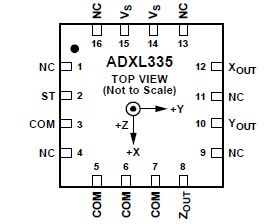
\includegraphics[scale=0.9]{figures/cProblemloesning/ADXL335.JPG}
	\caption{Accelerometeret ADXL335, hvor de forskellige indgange og udgange ses samt hvilken retning, som akserne forløber i. \cite{Devices2009}}
	\label{ADXL335}
\end{figure}

Når accelerometeret hældes til siden, vil der ske en acceleration ift. tyngdekraften i en given retning og dermed et udslag fra referencepunktet, som er ved en hældning på 0$^{\circ}$. Hvis accelerometeret f.eks. blev stillet på højkant, som det ses på \figref{ADXL335}, vil x aksen blive påvirket med -1 g.\cite{Devices2009} \\
Sammenhængen mellem de enkelte parametre kan udtrykkes ved følgende ligninger:\\ 
\begin{align}
	V_{out} = V_{offset} + sensitiviteten * tyngdekraften * \sin(vinklen) \\
	V_{out} = V_{offset} + \frac{\Delta V}{\Delta g} * g * \sin \Theta
\end{align}
Herudfra er det muligt at isolere og udregne de ukendte parametre, altså kan patientens hældningsgrad bestemmes ud fra accelerometerets output.

\subsection{Systemets opbygning}\label{ref:blokdiagram} \fxnote{Erika: strømforsyning?}
Systemets opbygning fremgår af \figref{kravblok}.

\begin{figure}[H]
	\centering
	\includegraphics[scale=0.5]{figures/cProblemloesning/Blokdiagram.PNG}
	\caption{Figuren viser de enkelte blokke, som systemet skal indeholde.}
	\label{kravblok}
\end{figure}
Det biologiske signal, der opnås fra accelerometeret, skal som det første filtreres vha. et lavpasfilter. Dette gøres for at frasortere uønskede frekvenser  over 45 Hz. Grunden til disse frekvenser kan frasorteres, er at det signal som skal måles ligger under 45 Hz. Efter filtreringen af signalet benyttes en variabel forstærker, for at tilpasse signalets amplitude til ADC’en og komparatoren. Signalet ledes herefter videre i et analogt og digitalt kredsløb. I det analoge kredsløb kommer signalet først gennem en komparator. Denne skal sammenligne signalet med en tærskelværdi, som udregnes ift. accelerometerets output ved måling på hældningsgraden af forsøgspersonen. Derved kan den rigtige feedback kan gives til patienten. Feedbacken bliver givet til patienten i form at dioder og vibratorer således, det muligvis bliver muligt for patienten at holde balancen bedre. I det digitale kredsløb, bliver signalet ledt ind i en ADC. Denne vil omdanne det analoge biologiske signal til et digitalt signal. Det digitale signal bliver herefter ledt ind i en USB-isolator, så der ikke opstår lækstrømme og for at sikre patientens sikkerhed. Til sidst vil det digitale signal overført til en computer, hvor signalet herefter vil kunne gemmes. Det bliver herved muligt at databehandle signalet og opstille det som en graf eller lignende. \\
Systemet har altså både et output henvendt til patienterne og det fagkyndige personale. Patienternes output er den feedback, der oplyser om deres hældningsgrad. Programmet, der skal behandle og gemme patienternes øvelsesresultater, er output til det fagkyndige personale. 
